%!TEX root = ../../thesis.tex
%*******************************************************************************
%****************************** Solution Implementation Chapter *********************************
%*******************************************************************************

\chapter{Solution Implementation}

\ifpdf
    \graphicspath{{Chapters/Implementation/Figs/}{Chapters/Implementation/Figs/}{Chapters/Implementation/Figs/}}
\else
    \graphicspath{{Chapters/Implementation/Figs/}{Chapters/Implementation/Figs/}}
\fi
In the previous chapter, we displayed an overview design of our approach.
Consequently, the solution implementation chapter of this thesis presents the details of how the proposed system was developed and implemented.
Firstly, we define some \ac{df} (see section \ref{implementation:section:designfeatures}) that focus on designing and developing new artifacts, methods, or systems.
It begins with a description of the system's architecture (see section \ref{implementation:section:architecture}), including the major components and their interactions.
Next, the description of the technology stack and development tools is explained (see section \ref{implementation:section:technologies}).
The chapter includes a detailed explanation of the critical features and functionality of the system and the processes used in frontend implementation (see section \ref{implementation:section:frontend}), database implementation (see section \ref{implementation:section:database}) backend implementation (see section \ref{implementation:section:backend}), and the software tool (see section \ref{implementation:section:tool}). 
Finally, the chapter discusses the challenges encountered during the implementation process and the lessons learned (see section \ref{implementation:section:challenges}). 
Through this chapter, readers will understand how we brought the proposed solution to reality and its potential for real-world applications.

\section{Platform Design Features (DFs)}
\label{implementation:section:designfeatures}
\ac{dsr} aims to produce a tangible outcome, such as a new software tool, a process improvement, or a theoretical framework.
It often involves multiple cycles of design, evaluation, and redesign, allowing for constant improvement of the artifact.
In this thesis, we perform the \textit{first} iteration of the cycle.
Using the \ac{df}s, we represent the features of our platform. 
\ac{df}s is used for the creation of a new artifact, method, or system.
Each \ac{dp}s is translated into a set of \ac{df}s that we can directly implement into the tool or platform.
In the following, we describe the \ac{df}s for each of the derived \ac{dp}s.

\begin{figure}[htbp!]
    \centering    
    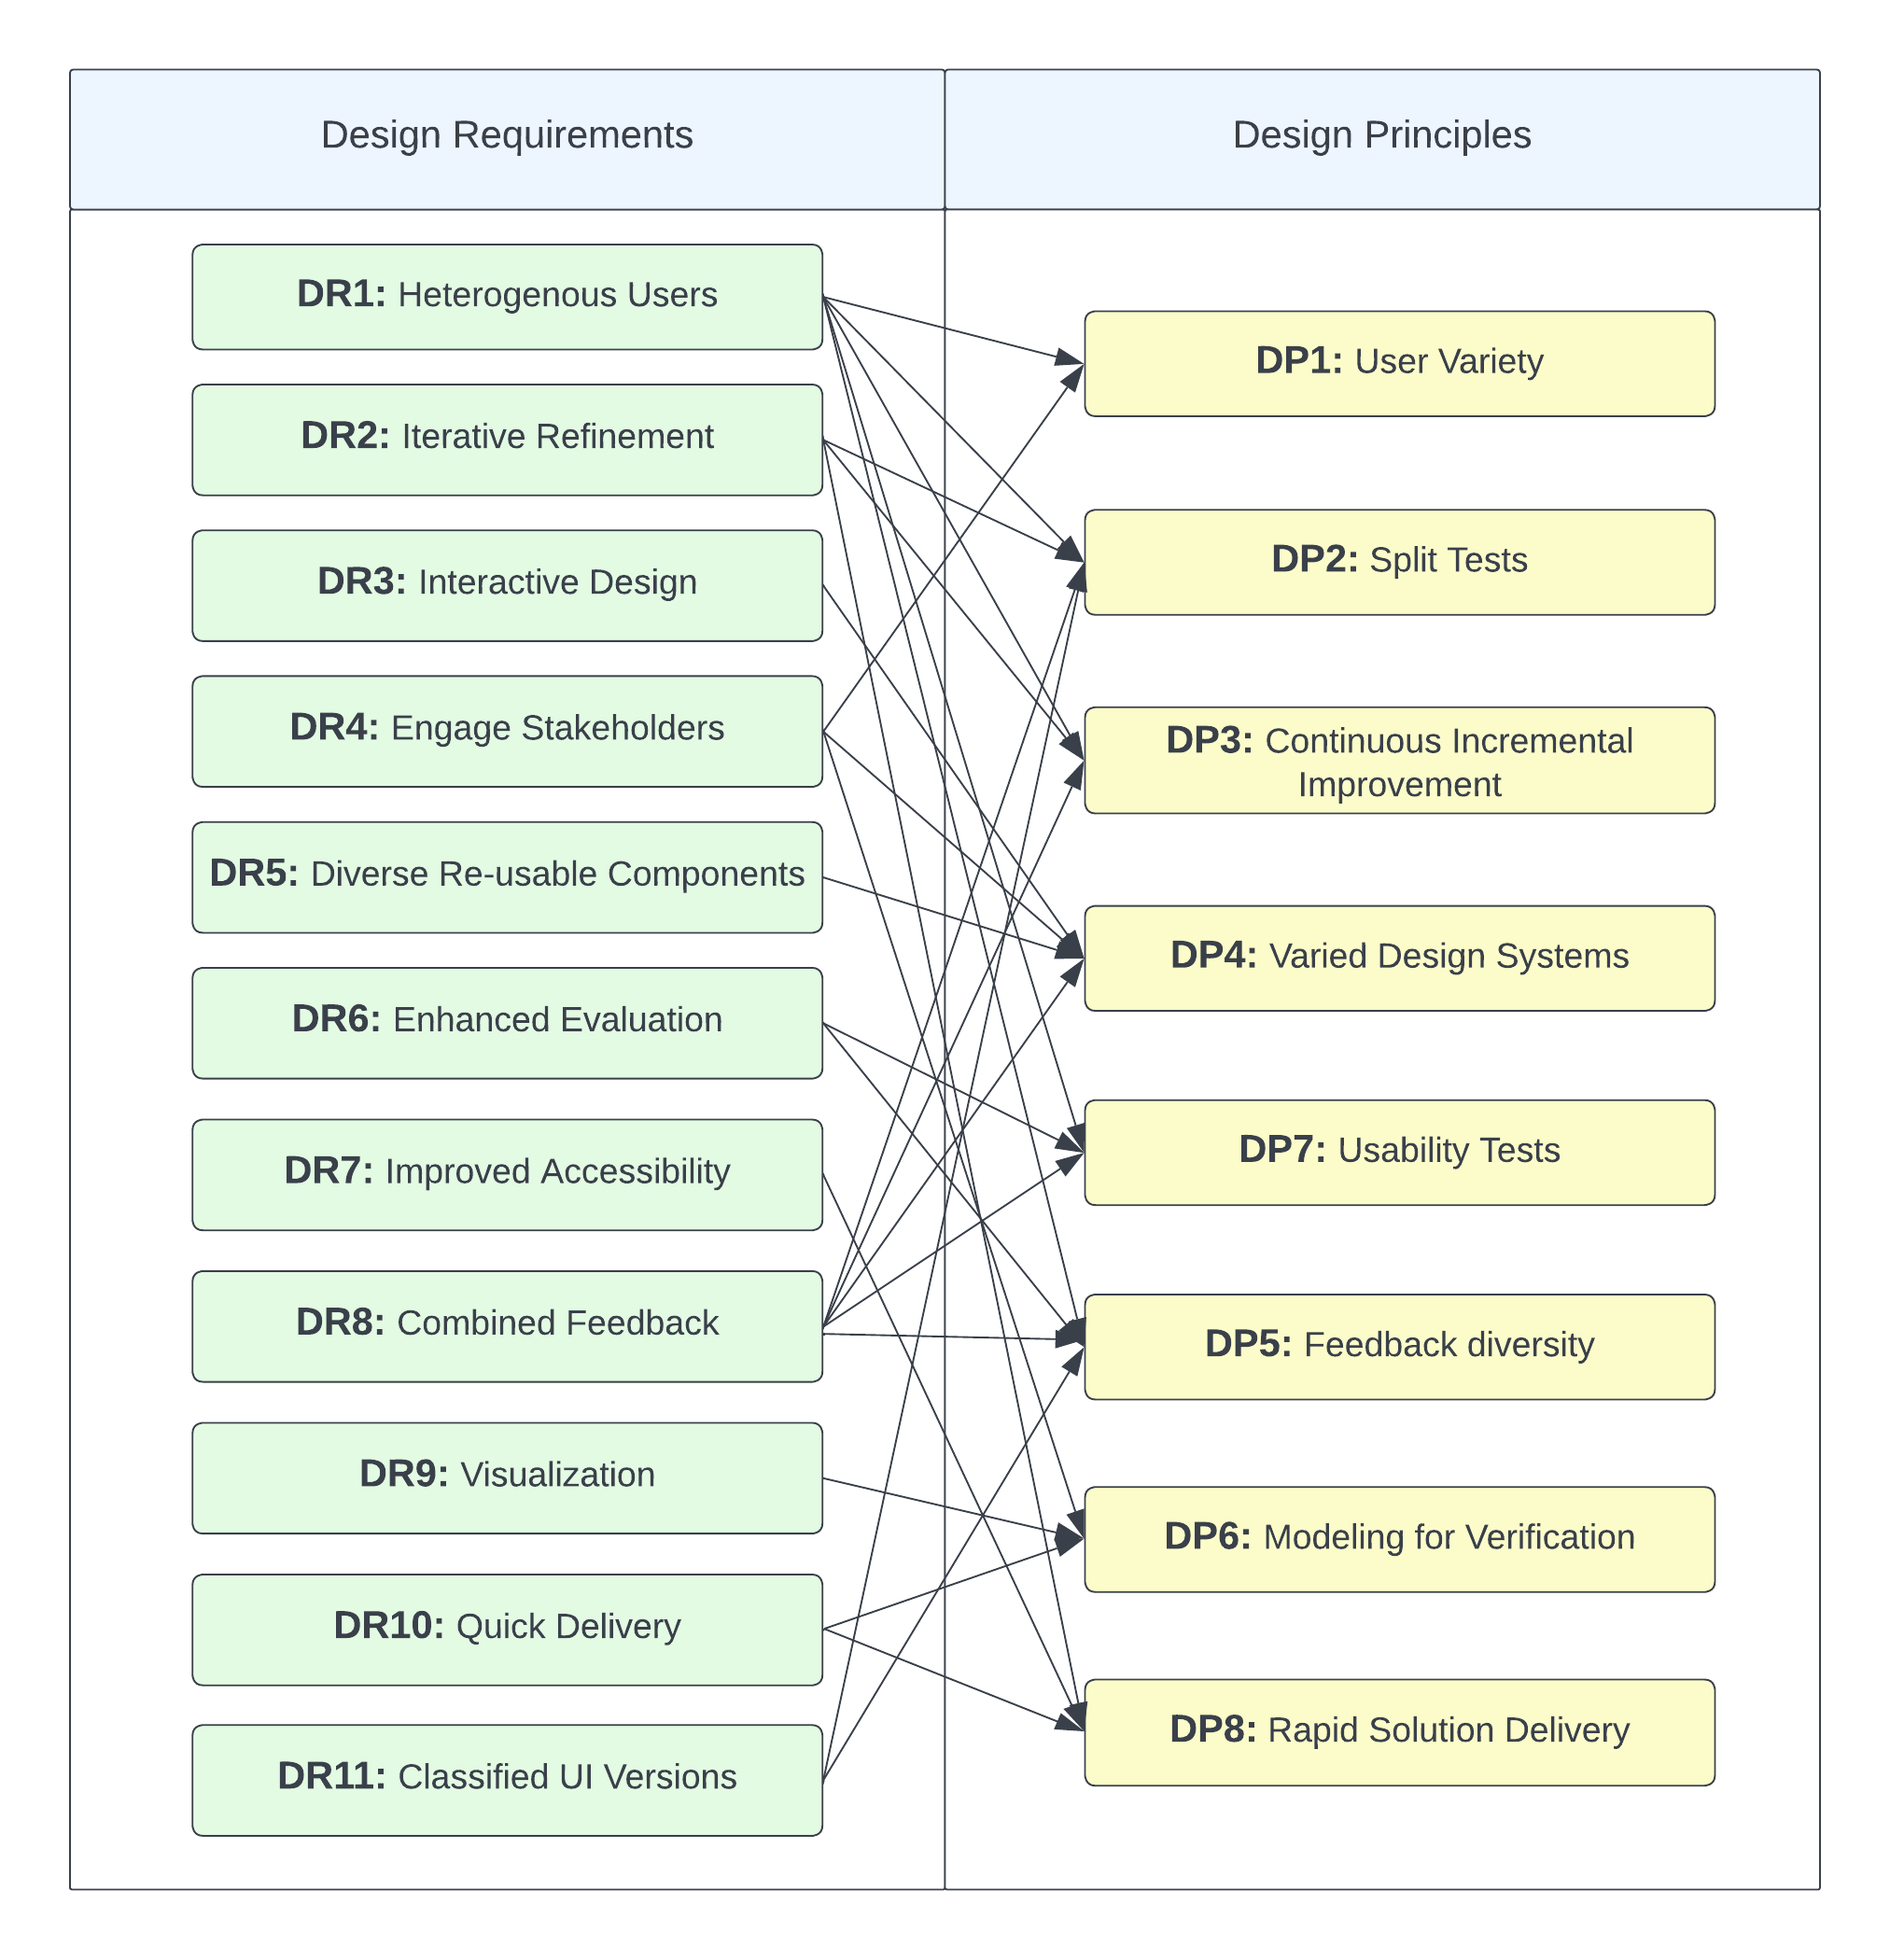
\includegraphics[width=0.8\textwidth]{Table-dps-dfs.png}
    \caption[A map between \ac{dp}s and \ac{df}s]{A map between Design Principles and Design Features}
    \label{fig:implementation:table-dps-dfs}
\end{figure}

\section{System Architecture}
\label{implementation:section:architecture}

\section{Technologies Used}
\label{implementation:section:technologies}

\section{Frontend Implementation}
\label{implementation:section:frontend}

\section{Database Schema}
\label{implementation:section:database}

\section{Backend Implementation}
\label{implementation:section:backend}

\section{Software Tool}
\label{implementation:section:tool}

\section{Encountered Challenges and Lessons Learnt}
\label{implementation:section:challenges}